\documentclass[article]{jss}

%% -- LaTeX packages and custom commands ---------------------------------------

%% recommended packages
\usepackage{thumbpdf,lmodern}

%% additional packages
\usepackage{amssymb,amsmath}

%% new custom commands
\newcommand{\class}[1]{`\code{#1}'}
\newcommand{\fct}[1]{\code{#1()}}
\raggedbottom

%% For Sweave-based articles about R packages:
%% need no \usepackage{Sweave}



%% -- Article metainformation (author, title, ...) -----------------------------

%% - \author{} with primary affiliation
%% - \Plainauthor{} without affiliations
%% - Separate authors by \And or \AND (in \author) or by comma (in \Plainauthor).
%% - \AND starts a new line, \And does not.
\author{Lennart Oelschl\"ager \\Bielefeld University \And Timo Adam \\University of St Andrews\And Rouven Michels \\Bielefeld University}
\Plainauthor{Lennart Oelschl\"ager, Timo Adam, Rouven Michels}

%% - \title{} in title case
%% - \Plaintitle{} without LaTeX markup (if any)
%% - \Shorttitle{} with LaTeX markup (if any), used as running title
\title{\pkg{fHMM}: Hidden Markov Models for Financial Time Series in \proglang{R}}
\Plaintitle{fHMM: Hidden Markov Models for Financial Time Series in R}
\Shorttitle{fHMM}

\Abstract{
%% Intro to HMMs
Hidden Markov models constitute a versatile class of statistical models for time series that are driven by hidden states. In financial applications, the hidden states can often be linked to market regimes such as bearish and bullish markets or recessions and periods of economics growth. To give an example, when the market is in a nervous state, corresponding stock returns often follow some distribution with relatively high variance, whereas calm periods are often characterized by another distribution with relatively smaller variance. Hidden Markov models can be used to explicitly model the distributions of the observations conditional on the hidden states and the transitions between states, and thus help us to draw a comprehensive picture of market behavior.
%% Intro to the package
In this paper, we introduce the \proglang{R} package \pkg{fHMM}, which provides various tools for applying hidden Markov models to financial time series. It provides functions for fitting hidden Markov models to empirical data, conducting simulation experiments, and decoding the underlying state sequence. Furthermore, functions for model checking, model selection, and state prediction are provided. In addition to basic hidden Markov models, hierarchical hidden Markov models are implemented. Its aim is to give \proglang{R} users interested in financial applications access to hidden Markov models and their extensions.
}

%% - \Keywords{} with LaTeX markup, at least one required
%% - \Plainkeywords{} without LaTeX markup (if necessary)
%% - Should be comma-separated and in sentence case.
\Keywords{hidden Markov models, regime switching, financial time series, decoding market behavior, \proglang{R}}
\Plainkeywords{hidden Markov models, regime switching, financial time series, decoding market behavior, R}

%% - \Address{} of at least one author
%% - May contain multiple affiliations for each author
%%   (in extra lines, separated by \emph{and}\\).
%% - May contain multiple authors for the same affiliation
%%   (in the same first line, separated by comma).
\Address{
  Lennart Oelschl\"ager\\
  Department of Business Administration and Economics\\
  Bielefeld University\\
  Postfach 10 01 31, Germany\\
  E-mail: \email{lennart.oelschlaeger@uni-bielefeld.de}\\ \\
  Timo Adam \\
  School of Mathematics and Statistics\\
  University of St Andrews\\
  The Observatory, Buchanan Gardens, St Andrews KY16 9LZ, UK\\
  E-mail: \email{ta59@st-andrews.ac.uk}\\ \\
  Rouven Michels \\
  Department of Business Administration and Economics\\
  Bielefeld University\\
  Postfach 10 01 31, Germany\\
  E-mail: \email{r.michels@uni-bielefeld.de}
}

\begin{document}
%% Do we need to following line?
%% \SweaveOpts{concordance=TRUE}

%% -- Introduction -------------------------------------------------------------

%% - In principle "as usual".
%% - But should typically have some discussion of both _software_ and _methods_.
%% - Use \proglang{}, \pkg{}, \fct{} and \code{} markup throughout the manuscript.
%% - If such markup is in (sub)section titles, a plain text version has to be
%%   added as well.
%% - All software mentioned should be properly \cite-d.
%% - All abbreviations should be introduced.
%% - Unless the expansions of abbreviations are proper names (like "Journal
%%   of Statistical Software" above) they should be in sentence case (like
%%   "generalized linear models" below).

\section{Introduction}
\label{sec:intro} %% Timo 

%% Intro to HMMs
In recent years, Hidden Markov models (HMMs) have emerged as a popular tool for modeling time series that are subject to state-switching over time \citep{zuc16}. In their basic form, HMMs comprise an observed state-dependent process that is driven by a hidden state process, the latter of which is typically modeled using a discrete-time, finite-state Markov chain. In financial applications, the states of the underlying Markov chain can often be linked to market regimes such as bearish and bullish markets or recessions and periods of economics growths. To give an example, when the market is in a nervous state, corresponding stock returns often follow some distribution with relatively high variance, whereas when the market is in a clam state, another distribution with relatively smaller variance is active. By their dependence structure, HMMs naturally account for such disparate patterns and thus allow us to infer hidden market regimes and their underlying dynamics from financial time series.

%% Literature review
Over the last decades, HMMs have become increasingly popular in finance. In various studies, they have been applied to model business cycles \citep{kim98, gre00}, to derive stylized facts of stock returns \citep{bul06, nys15a}, and to model energy prices conditional on market regimes \citep{lan18, ada19c, ada22}, to name but a few examples. \cite{lih17} used HMMs to model volatility in the Standard and Poor's 500 index to investigate the conjecture that stock returns exhibit negative correlation with volatility. \cite{ngu18} used HMMs to predict closing prices to derive an optimal trading strategy, which was shown to outperform the conventional buy-and-hold strategy, whereas \cite{bul11, nys15a, nys18} have shown that HMMs prove useful in asset allocation and portfolio optimization applications. All these examples demonstrate that HMMs constitute a versatile class of statistical models for time series that naturally accounts for the state-switching patterns often found in financial data.

%% Software overview
In \proglang{R} \citep{r21}, various implementations of HMMs are available. For general purposes, the packages \pkg{hmm} \citep{him10}, \pkg{depmixS4} \citep{vis10}, and \pkg{msm} \citep{jac11} are frequently used. In addition, a wide range of special-purpose packages is available, for example \pkg{moveHMM} \citep{mic16} and \pkg{momentuHMM} \citep{mcc18} for modeling ecological time series, \pkg{hsmm} \citep{bul10} and \pkg{mhsmm} \citep{oco11} for hidden semi-Markov models, \pkg{hmm.discnp} \citep{tur14} and \pkg{countHMM} \citep{ada19b} for modeling count data, and \pkg{LMest} \citep{bar17} for modeling longitudinal data. In \proglang{Python}, the library \pkg{hmmlearn} \citep{leb22} can be used. Yet, an \proglang{R} package tailored to financial applications is still lacking.

%% Intro to the package
In this paper, we introduce the \proglang{R} package \pkg{fHMM} \citep{oel22}, which aims to complement the above mentioned collection by making HMMs accessible to \proglang{R} users with a special interest in financial time series. The package functionality can be classified into functions for data preparation, model estimation, and model evaluation, which are illustrated in the flowchart displayed in Figure \ref{fig:flowchart}. 
\begin{figure}[t!]
  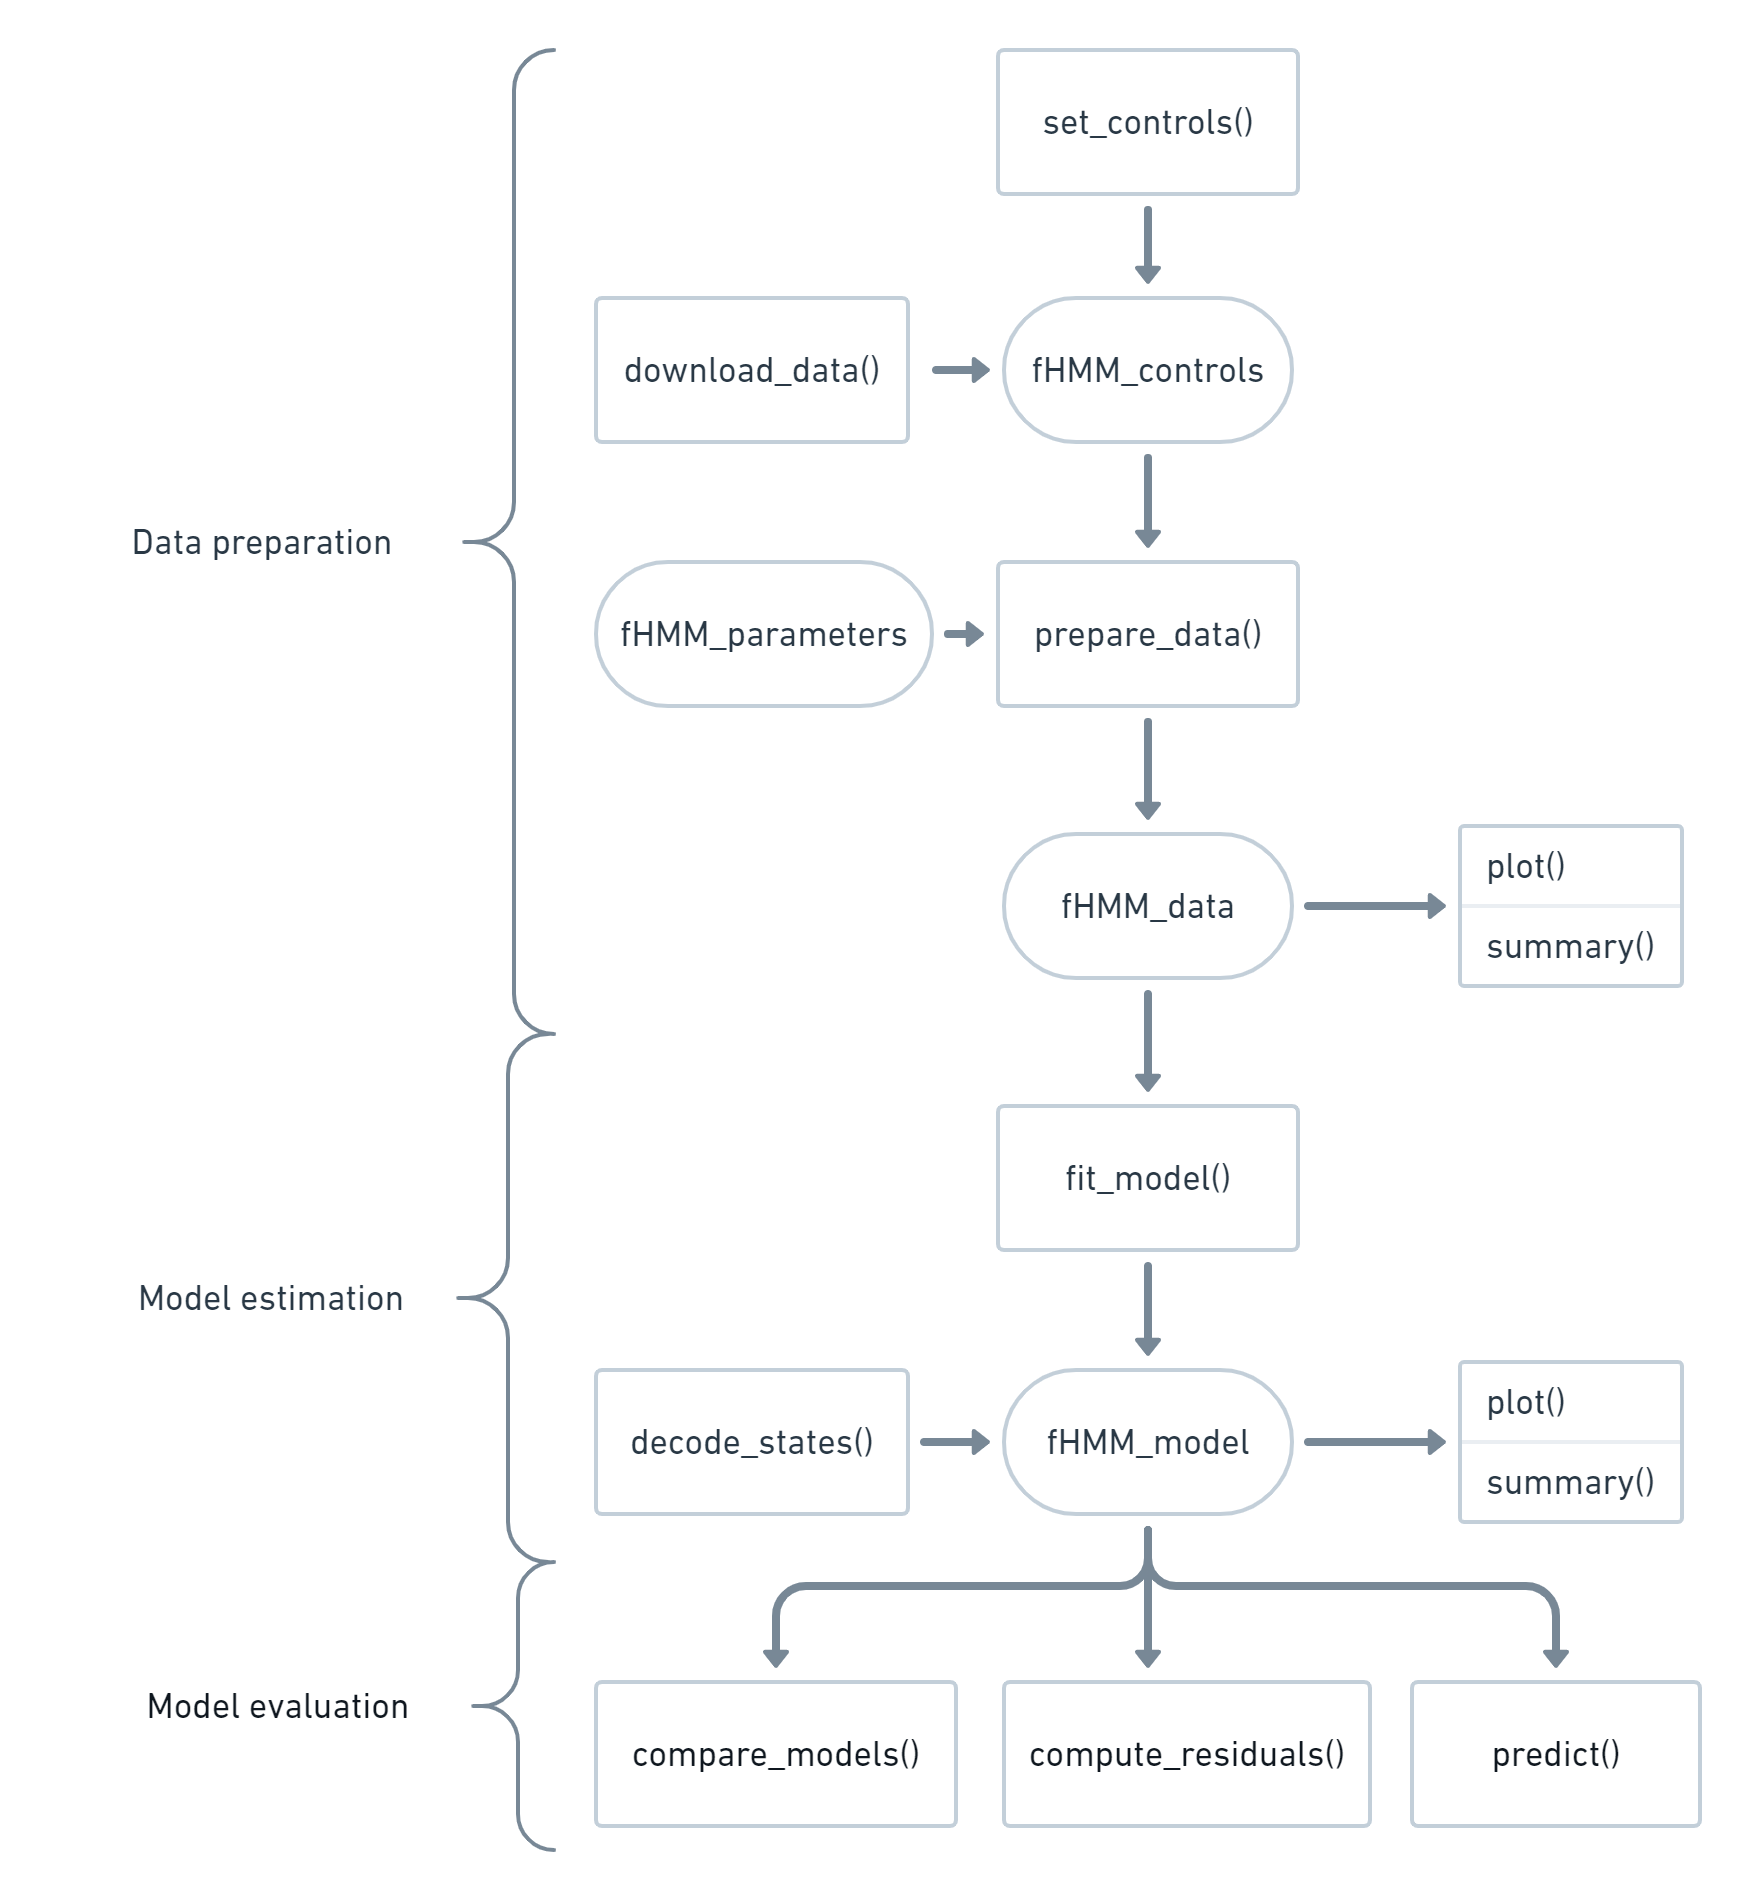
\includegraphics{flowchart.png}
  \caption{Package flowchart. The main functions are visualized using rectangles, while objects are illustrated as ovals.}
  \label{fig:flowchart}
\end{figure}
Functions for data preparation include a convenient interface to Yahoo Finance (https://www.finance.yahoo.com) that allows users to download stock market data. The model is estimated in a maximum likelihood framework, where the likelihood is evaluated using the forward algorithm, which is implemented in \proglang{C++} and parallelized for fast and efficient computation. Functions for model evaluation include pseudo-residual analyses and the computation of model selection criteria. The package also implements hierarchical HMMs (HHMMs); an extension of basic HMMs proposed in \cite{oel21} that improves the model's capability of distinguishing between short- and long-term trends and allows us to jointly model data streams collected at different time scales, such as monthly trade volumes and daily stock returns \citep{ada20}. 

%% Outline of the paper
The paper is structured as follows: in Section \ref{sec:model_definition}, we introduce HMMs and HHMMs, focusing on their dependence structure and model assumptions. In Sections \ref{sec:model_specification}--8, we illustrate a typical workflow using the \pkg{fHMM} package, where we explain how to specify the model, how to download, prepare, and simulate data, how to fit the model, how to decode the hidden states, how to use a fitted model for state forecasting, how to check the goodness of fit, and how to perform model selection. Each section begins with some theoretical background, which is followed by illustrating examples using simulated data, stock index data from the Deutscher Aktienindex (DAX), and stock market data from the Volkswagen Group (VW). Each of these sections is complemented by code chunks, which cannot only be used to replicate the examples given but also serve as a starting point for \proglang{R} users interested in financial time series who want to apply HMMs to their own data. Section \ref{sec:conclusion} concludes and gives an outlook of anticipated, future package extensions.

%% -- Manuscript ---------------------------------------------------------------

%% - In principle "as usual" again.
%% - When using equations (e.g., {equation}, {eqnarray}, {align}, etc.
%%   avoid empty lines before and after the equation (which would signal a new
%%   paragraph.
%% - When describing longer chunks of code that are _not_ meant for execution
%%   (e.g., a function synopsis or list of arguments), the environment {Code}
%%   is recommended. Alternatively, a plain {verbatim} can also be used.
%%   (For executed code see the next section.)
%% - Tables are placed at the top of the page
%%   (\verb|[t!]|), centered (\verb|\centering|), with a caption below the table,
%%   column headers and captions in sentence style, and if possible avoiding
%%   vertical lines.
%% - Virtually all JSS manuscripts list source code along with the generated
%%   output. The style files provide dedicated environments for this.
%% - In R, the environments {Sinput} and {Soutput} - as produced by Sweave() or
%%   or knitr using the render_sweave() hook - are used (without the need to
%%   load Sweave.sty).
%% - Equivalently, {CodeInput} and {CodeOutput} can be used.
%% - The code input should use "the usual" command prompt in the respective
%%   software system.
%% - For R code, the prompt "R> " should be used with "+  " as the
%%   continuation prompt.
%% - Comments within the code chunks should be avoided - these should be made
%%   within the regular LaTeX text.
%% - Please make sure that all code is properly spaced, e.g., using
%%   \code{y = a + b * x} and \emph{not} \code{y=a+b*x}.
%% - JSS prefers when the second line of code is indented by two spaces.

\section{Model definition} \label{sec:model_definition} %% Rouven

Hidden Markov models (HMMs) constitute a modeling framework for time series where a sequence of observations is assumed to depend on a hidden state process. The peculiarity is that, instead of the observation process, the state process cannot be directly observed. However, the hidden states comprise information about the environment the model is applied on. The hidden state process and the observed state-dependent process are connected as follows: we assume that for each point in time $t = 1, \ldots, T$, an underlying process $(S_t)_{t = 1, \ldots, T}$ is in one of $N$ possible states. Then, depending on the active state $S_t \in \{ 1, \ldots, N \}$, the observation $X_t$ from the state-dependent process $(X_t)_{t = 1, \ldots, T}$ is assumed to be generated by the corresponding state-dependent distribution $f^{(S_t)}$. We assume $(S_t)_t$ to be Markovian, i.e.\ the active state at time $t$ only depends on the previous state at time $t-1$. Henceforth, the state process is identified by its initial distribution $\delta = (\delta_i), \delta_i = \Pr(S_1 = i), i = 1, \ldots, N$, and its transition probability matrix (t.p.m.) $\Gamma = (\gamma_{i,j}), \gamma_{i,j} = \Pr(S_{t} = j|S_{t-1}=i), i,j = 1, \ldots, N, t = 2, \ldots, T$. Furthermore, $(X_t)_{t = 1, \ldots, T}$ satisfies the conditional independence assumption, i.e.\ the observation $X_t$ depends on the current state $S_t$, but is independent from previous observations or states.

When modeling financial time series, the different states can serve as proxies for the current market situation, e.g.\ calm and nervous. Even though these moods cannot be directly observed, price changes or trading volumes (which can be assumed to depend on the current mood of the market) are observable. Thereby, using an underlying Markov process, we can detect which mood is active at any point in time and how the different moods alternate. Depending on the current mood, a price change is generated by a different distribution. These distributions characterize the moods in terms of expected return and volatility. For example, we can explicitly model price changes at time $t$ by different normal distributions whose mean and variance depend on the current state, $S_t$.

Following \cite{zuc16}, we assume that the initial distribution $\delta$ equals the stationary distribution $\pi$, where $\pi = \pi \Gamma$, i.e.\ the stationary and henceforth the initial distribution is determined by $\Gamma$.\footnote{A note on the existence of a stationary distribution: If the Markov process is irreducible, it has a unique distribution, which is the solution to the equation system $\pi = \pi \Gamma$. If, additionally, the Markov process is aperiodic, its state distribution converges to the stationary distribution, see \cite{nor97}. Irreducibility and aperiodicity are usually satisfied in practice.} This is reasonable from a practical point of view: On the one hand, the hidden state process has been evolving for some time before we start to observe it and hence can be assumed to be stationary. On the other hand, setting $\delta=\pi$ reduces the number of parameters that need to be estimated, which is convenient from a computational perspective.

HHMMs constitute a flexible extension of the basic HMM that can jointly model data observed on two different time scales \citep{oel21}. The two time series, one on a coarser and one on a finer scale, differ in the number of observations, e.g.\ monthly observations on the coarser scale and daily observations on the finer scale. Following the concept of HMMs, we can model both state-dependent time series jointly. First, we treat the time series on the coarser scale as stemming from an ordinary HMM, which we refer to as the coarse-scale HMM: At each time point $t$ of the coarse-scale time space $\{1,\dots,T\}$, an underlying process $(S_t)_t$ selects one state from the coarse-scale state space $\{1,\dots,N\}$. We refer to $(S_t)_t$ as the hidden coarse-scale state process. Depending on which state is active at time $t$, one of $N$ possible distributions $f^{(1)},\dots,f^{(N)}$ realizes the observation $X_t$. The process $(X_t)_t$ is called the observed coarse-scale state-dependent process. The processes $(S_t)_t$ and $(X_t)_t$ have the same properties as before, namely $(S_t)_t$ is a first-order Markov process and $(X_t)_t$ satisfies the conditional independence assumption. This dependence structure is visualized in the upper part of Figure \ref{fig:hhmm}.

For the fine-scale time series, the observed data is split into $T$ distinct chunks, each of them having a correspondence to the $t$-th coarse scale time point. So, the hierarchical structure arises naturally: for each chunk, we model the containing data points via the fine-scale HHM, which is selected by the hidden coarse-scale state $S_t$. Thus, each fine-scale HMM consists of two stochastic processes: the hidden, fine-scale process $(S^*_{t,t^*})_{t^*}$ selecting states from $\{1,\dots,N^*\}$, the fine-scale state space, for each time point $t^*$ in $\{1,\dots,T^*\}$, the fine-scale time space and the observed, fine-scale process $(X^*_{t,t^*})_{t^*}$ whose observations are assumed to depend on one of $N^*$ possible distributions $f^{*(i,1)},\dots,f^{*(i,N^*)}$, chosen depending on the actual state of the hidden, fine-scale process. By construction, each fine-scale HMM contains of an own t.p.m.\ $\Gamma^{*(i)}$, initial distribution $\delta^{*(i)}$, stationary distribution $\pi^{*(i)}$, and state-dependent distributions $f^{*(i,1)},\dots,f^{*(i,N^*)}$. Similar to the coarse-scale HMM, the hidden, fine-scale process is Markovian and satisfies the conditional independence assumption. In contrast, the observed, fine-scale process has exclusive dependence on the actual state of the hidden, fine-scale process. In the lower part of Figure \ref{fig:hhmm}, the dependence and hierarchical structure is visualized.

\begin{figure}
  \centering
  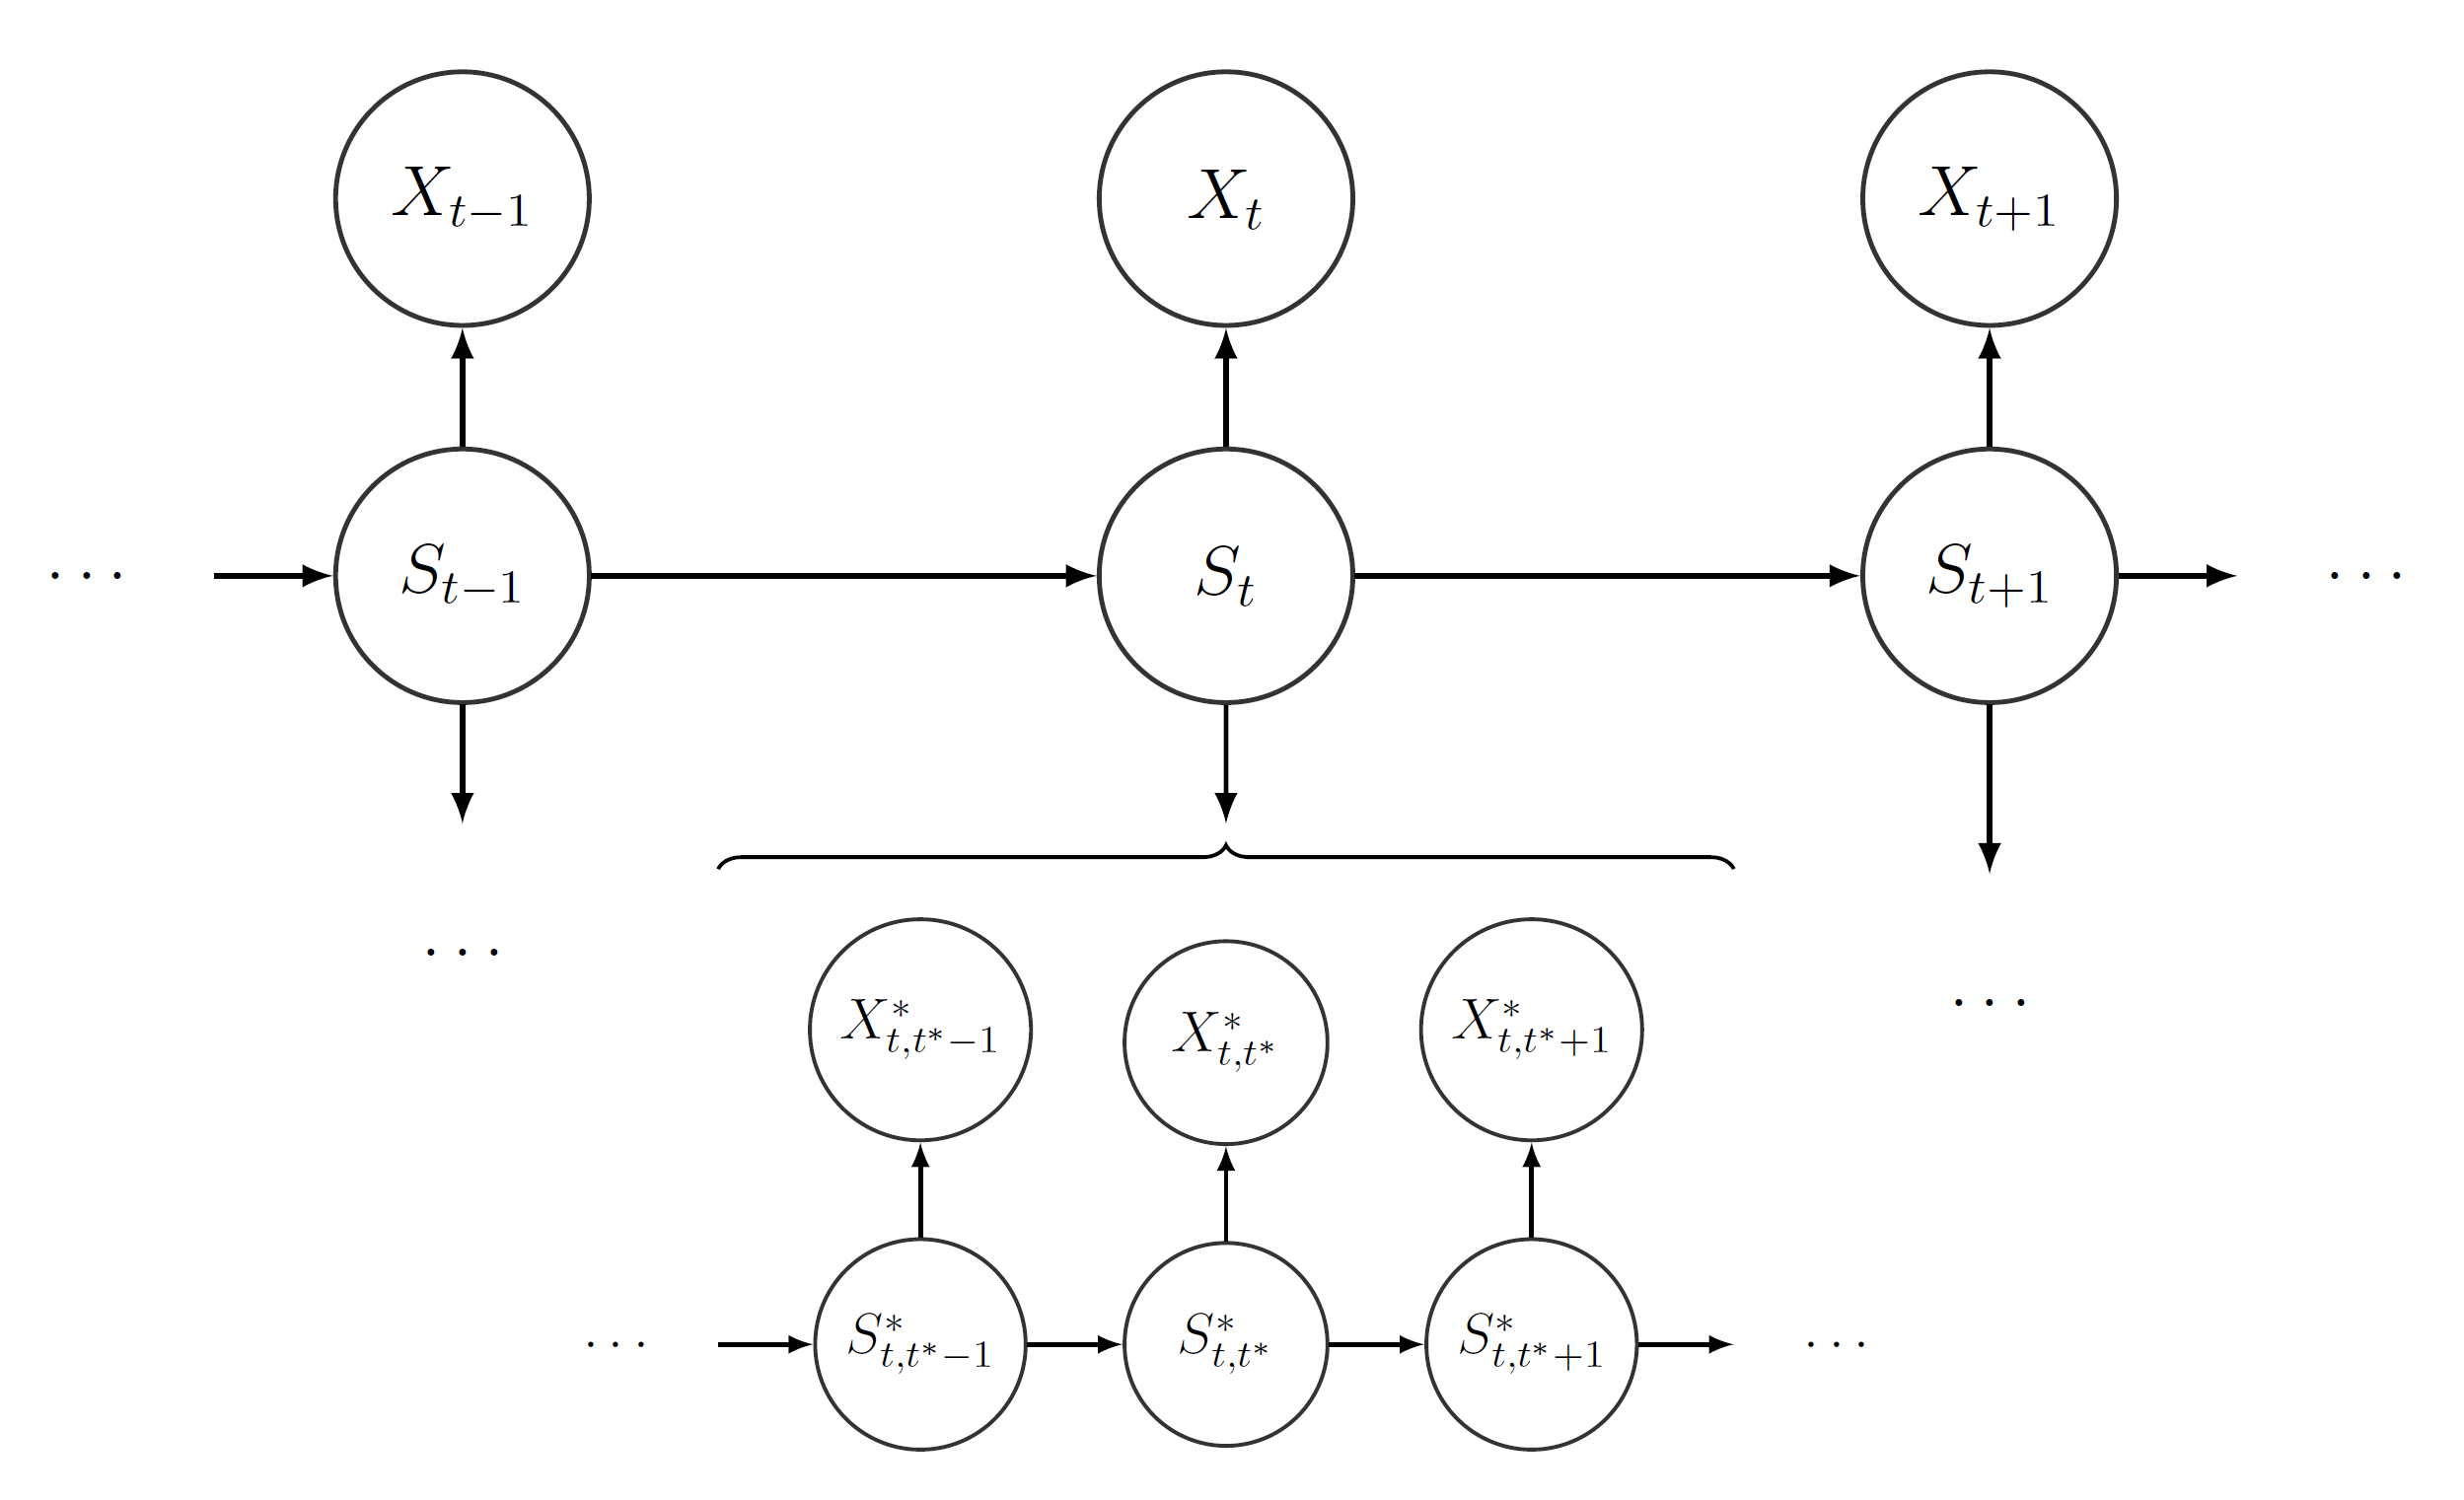
\includegraphics{hhmm.png}
  \caption{Dependence structure of an HHMM. The dependence structure of a basic HMM is visualized in the upper part.}
  \label{fig:hhmm}
\end{figure}

\section{Model specification} \label{sec:model_specification} %% Lennart

In the \pkg{fHMM} package, models are specified by a named list of controls that is passed to the \fct{set\_controls} function. This usually constitutes the first step when using the package, see Figure \ref{fig:flowchart}. The function checks the specifications and returns an \class{fHMM\_controls} object, which stores all settings and thereby provides the information required for other functionalities. In the following, we demonstrate three example specifications that should help the user to tailor an HMM to their need. The examples are continued in the following sections. All possible specifications are documented in detail on the function's help page, which can be accessed from the \proglang{R} console via \code{help(set_controls, package = "fHMM")}.

\paragraph{Example 1: DAX.} We fit a 3-state HMM to the closing prices of the DAX \citep{jan92}. Assume that the time series data is available in the working directory as file \code{"dax.csv"}. Such data can be obtained directly from Yahoo Finance via the convenience function \fct{download\_data}, see Section \ref{sec:data_management}.

The following lines set the number \code{states = 3} of hidden states. Any number greater than or equal to 2 is possible. Next, \code{sdds = "t"} specifies state-dependent t-distributions, which provides a popular choice for modeling log-returns \citep{pla08}. Alternatively, \code{sdds = "gamma"} specifies Gamma distributions, which is useful for model trading volumes as in \cite{ada20}. The \code{data} entry sets the path to the data file (\code{file = "dax.csv"}), the file's column that contains the dates (\code{date_column = "Date"}), and the data (\code{date_column = "Close"}). The specification \code{logreturns = TRUE} transforms the data to log-returns.

%
\begin{Schunk}
\begin{Sinput}
R> contr_dax <- list(
+    states = 3,
+    sdds   = "t",
+    data   = list(file        = "dax.csv",
+                  date_column = "Date",
+                  data_column = "Close",
+                  logreturns  = TRUE)
+  )
\end{Sinput}
\end{Schunk}
%

Passing this list to the \fct{set\_controls} function returns an object of class \class{fHMM\_controls}, which contains the specifications and default settings.

%
\begin{Schunk}
\begin{Sinput}
R> contr_dax <- set_controls(contr_dax)
R> class(contr_dax)
\end{Sinput}
\begin{Soutput}
[1] "fHMM_controls"
\end{Soutput}
\end{Schunk}
%

\paragraph{Example 2: Simulation.} If the \code{data} entry is not specified, data will be simulated according to the model specification. Simulation typically serves to assess the properties of estimation algorithms either for research or in a bootstrap-like fashion, as can be seen for example in \cite{oel19}. The following code chunk specifies a 2-state HMM with state-dependent Gamma distributions, where the expected values for state 1 and 2 are fixed to \code{1} and \code{2}, respectively. The model is fitted to 200 data points (\code{horizon = 200}) simulated according to this specification based on \code{runs = 50} randomly initialized numerical optimization runs of the model's likelihood function. Printing the \class{fHMM\_controls} object summarizes the model specification:

%
\begin{Schunk}
\begin{Sinput}
R> contr_sim <- list(
+    states  = 2,
+    sdds    = "gamma(mu = 1|2)",
+    horizon = 200,
+    fit     = list(runs = 50)
+  )
R> (contr_sim <- set_controls(contr_sim))
\end{Sinput}
\begin{Soutput}
fHMM controls:
* hierarchy: FALSE 
* data type: simulated 
* number of states: 2 
* sdds: gamma(mu = 1|2) 
* number of runs: 50  
\end{Soutput}
\end{Schunk}
%

\paragraph{Example 3: Hierarchy.} An HHMM can be specified by adding \code{hierarchy = TRUE} to the controls. The following is a specification for the DAX on the fine scale and the VW stock on the coarse scale (both data sets are contained in the \pkg{fHMM} package): 

%
\begin{Schunk}
\begin{Sinput}
R> contr_hhmm <- list(
+    hierarchy = TRUE,
+    states    = c(2,2),
+    sdds      = c("t(df = 1)", "t(df = 1)"),
+    period    = "m",
+    data      = list(file = c(system.file("extdata", "dax.csv", package = "fHMM"),
+                              system.file("extdata", "vw.csv", package = "fHMM")),
+                     date_column = c("Date","Date"),
+                     data_column = c("Close","Close"),
+                     from = "2015-01-01",
+                     to = "2020-01-01",
+                     logreturns = c(TRUE,TRUE),
+                     merge = function(x) mean(x))
+  )
R> contr_hhmm <- set_controls(contr_hhmm)
\end{Sinput}
\end{Schunk}
%

The line \code{states = c(2, 2)} specifies \code{2} coarse-scale and \code{2} fine-scale states, respectively. State-dependent t-distributions are used, where the degrees of freedom are fixed to \code{1} on both scales (setting \code{df = Inf} is possible and would result in state-dependent normal distributions). Via \code{period = "m"}, we specify a monthly fine-scale time horizon. Alternatives are \code{"w"}, \code{"q"}, and \code{"y"} for weekly, quarterly, and yearly periods, respectively. The observation period is restricted to five years via \code{from = "2015-01-01"} and \code{to = "2020-01-01"}. With \code{logreturns = c(TRUE,TRUE)}, we ensure that the data on both scales are transformed to log-returns. If the coarse-scale data has a finer temporal resolution than defined by \code{period}, the data can be merged by specifying a function via the \code{merge} argument. In this example, the file \code{"dax.vw"} contains daily closing prices. Since we specified \code{merge = function(x) mean(x)}, the monthly average closing prices are used as coarse-scale observations.

\section{Data management} \label{sec:data_management} %% Lennart

Empirical data for modeling must be provided as a comma-separated values (.csv) file and its path must be specified in \fct{set\_controls}, see the previous section. The package includes the convenience function \fct{download\_data} for downloading daily stock market data directly from Yahoo Finance in the required format. The function call is \code{download\_data(symbol, from, to, file)}, where

- \code{symbol} is the stock's symbol that has to match the official symbol on Yahoo Finance,

- \code{from} and \code{to} define the desired time interval (in the format \code{"YYYY-MM-DD"}),

- \code{file} is the name of the saved file. Per default, it is saved in the current working directory under the name \code{<symbol>.csv}.

For example, the 21st century data of the DAX can be downloaded via the following line:

%
\begin{Schunk}
\begin{Sinput}
R> download_data(symbol = "^GDAXI", from = "2001-01-01", to = Sys.Date())
\end{Sinput}
\end{Schunk}
%

\paragraph{Example 1: DAX (cont.).} Recall the control specification for the 3-state HMM DAX model from the previous section. The \fct{prepare\_data} function prepares the data based on the specifications and returns an \class{fHMM\_data} object. This object can then be passed to the \fct{fit\_model} function for model fitting in the next step, see Section \ref{sec:model_estimation}. The \fct{summary} method provides a data overview.

%
\begin{Schunk}
\begin{Sinput}
R> data_dax <- prepare_data(contr_dax)
R> summary(data_dax)
\end{Sinput}
\begin{Soutput}
Summary of fHMM empirical data
* number of observations: 8828 
* data source: dax.csv 
* date column: Date 
* log returns: TRUE 
\end{Soutput}
\end{Schunk}
%

Additionally, the data can be visualized via the \fct{plot} method. To facilitate interpretation, historical events with a potential influence on the time series can be highlighted as follows:

%
\begin{Schunk}
\begin{Sinput}
R> events <- fHMM_events(
+    list(
+      dates = c("2001-09-11", "2008-09-15", "2020-01-27"),
+      labels = c("9/11 terrorist attack", "Bankruptcy of Lehman Brothers", 
+                 "First COVID-19 case in Germany")
+      )
+    )
R> plot(data_dax, events = events)